\documentclass[journal,12pt,twocolumn]{IEEEtran}
\usepackage[none]{hyphenat}
\usepackage{graphicx}
\usepackage{listings}
\usepackage[english]{babel}
\usepackage{graphicx}
\usepackage{caption} 
\usepackage{amsmath}
\usepackage{hyperref}
\usepackage{booktabs}
\usepackage{array}
\usepackage{stix}


\title{\textbf{\\Line Assignment}}
\author{kanekal kousar}
\date{September 2022}
\begin{document}
\maketitle


\section{Question}
\textbf{\textit{Class 11, Exercise 10.1, Q(9):} Without using distance formula, show that points (– 2, – 1), (4, 0), (3, 3) and (–3, 2)are the vertices of a parallelogram.}

\section{Solution}
\raggedright 

\begin{figure}[h!]
\centering
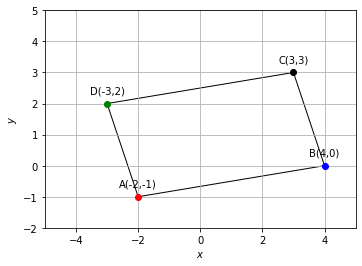
\includegraphics[scale=0.5]{fig/paralellogram.png} 
\caption{paralellogram ABCD}
\end{figure}

\vspace{0.25cm}
We can prove that the points are the vertices of a parallelogram if  \textbf{$\vec{AB}$} || \textbf{$\vec{DC}$} , \textbf{$\vec{BC}$} || \textbf{$\vec{AD}$} and  \textbf{$\vec{AB}$} =\textbf{$\vec{DC}$} , \textbf{$\vec{BC}$} = \textbf{$\vec{AD}$}
\vspace{0.3cm}

\textbf{Theorm:}if $\theta$ is the angle between $\vec{a}$ and $\vec{b}$,then

\hspace{3cm}
\boldmath
	$|\vec{a}\times \vec{b}|=|\vec{a}|| \vec{b}|cos\theta$
\unboldmath
\vspace{0.25cm}
\textbf{corollary:}The two non-zero vectors $\vec{a}$ and $\vec{b}$ are parallel to each other,if their product is a zero vector


Consider  Parallelogram ABCD,where

$ \vec{A}$ =$\begin{pmatrix}-2 \\ -1 \\ \end{pmatrix}$ \hspace{0.3cm} $ \vec{B} $=$\begin{pmatrix} 4\\ 0 \\ \end{pmatrix}$ 

$ \vec{C} $=$\begin{pmatrix}3 \\ 3 \\ \end{pmatrix}$ \hspace{0.3cm} $ \vec{D} $=$\begin{pmatrix}-3 \\ 2 \\ \end{pmatrix}$ 
\vspace{0.2cm}


let

$ \vec{P} =\vec{B}-\vec{A}=\begin{pmatrix}6 \\ 1 \\ \end{pmatrix}$ \hspace{0.3cm}$ \vec{Q}= \vec{C}-\vec{D}=\begin{pmatrix}6 \\ 1 \\ \end{pmatrix}$ 

$ \vec{R} = \vec{A}-\vec{C}=\begin{pmatrix}1 \\ -3 \\ \end{pmatrix}$ \hspace{0.3cm}$ \vec{S}= \vec{A}-\vec{D}=\begin{pmatrix}1 \\ -3 \\ \end{pmatrix}$ 

\subsection{\underline{proof for  \textbf{$\vec{P}$} || \textbf{$\vec{Q}$} and \textbf{$\vec{P}$} =\textbf{$\vec{Q}$}}}
\boldmath
$ \vec{P}\times \vec{Q}=|(\vec{B}-\vec{A})\times (\vec{C}-\vec{D}))|$
$ = \begin{vmatrix}
           \hat{i} & \hat{j}\\
            6 & 1\\
            6 & 1
    \end{vmatrix} = {0\hat{k}}  $
\unboldmath  
\vspace{0.2cm}
so,according to corollary $\vec{P} || \vec{Q}$

\boldmath
\begin{eqnarray}
||\vec{P}||=|1|+|6|=7
\end{eqnarray}
\begin{eqnarray}
||\vec{Q}||=|1|+|6|=7
\end{eqnarray}
\unboldmath

form equation (1) and (2) $\vec{P} = \vec{Q}$

\subsection{\underline{proof for  \textbf{$\vec{R}$} || \textbf{$\vec{S}$} and \textbf{$\vec{R}$} = \textbf{$\vec{S}$}}}
\boldmath
$\vec{R}\times \vec{S}=|(\vec{B}-\vec{C})\times (\vec{A}-\vec{D})|$
$ = \begin{vmatrix}
           \hat{i} & \hat{j}\\
            1 & -3\\
            1 & -3
    \end{vmatrix} = {0\hat{k}}  $
\unboldmath
\vspace{0.3cm}
so,according to corollary $\vec{R} || \vec{S}$
\boldmath
\begin{eqnarray}
||\vec{R}||=|1|+|-3|=4
\end{eqnarray}
\begin{eqnarray}
||\vec{S}||=|1|+|-3|=4
\end{eqnarray}
\unboldmath
form equation (3) and (4) $\vec{R} = \vec{S}$
\vspace{0.2cm}

since the opposite lines are parallel and equal the points (– 2, – 1), (4, 0), (3, 3) and (–3, 2) forms the vertices of a parallelogram

\section*{Construction}
\centering
\vspace{0.2cm}
{
\setlength\extrarowheight{2pt}
\begin{tabular}{|c|c|c|}
	\hline
	\textbf{Symbol}&\textbf{Value}&\textbf{Description}\\
	\hline
	$\vec{A}$ & $\begin{pmatrix}-2 \\ -1 \\ \end{pmatrix}$ & Vertex A\\
	\hline
	$\vec{B}$ & $\begin{pmatrix}4 \\ 0 \\ \end{pmatrix}$ & Vertex B\\
	\hline
	$\vec{C}$& $\begin{pmatrix}3 \\ 3 \\ \end{pmatrix}$ & Vertex C\\
	\hline
	$\vec{D}$ & $\begin{pmatrix}-3 \\ 2 \\ \end{pmatrix}$ & Vertex D\\
	\hline
	$\vec{P}$ &$\begin{pmatrix}1 \\ 6 \\ \end{pmatrix}$&vector AB\\
	\hline
	$\vec{Q}$ &$\begin{pmatrix}1 \\ 6 \\ \end{pmatrix}$&vector DC\\
	\hline
	$\vec{R}$ &$\begin{pmatrix}1 \\ -3 \\ \end{pmatrix}$&vector BC\\
	\hline
	$\vec{S}$ &$\begin{pmatrix}1 \\ -3 \\ \end{pmatrix}$&vector AD\\
	\hline
\end{tabular}
}

\vspace{0.6cm}
Get the python code of the figures from
\begin{table}[h]
\large
\centering
\framebox{
\url{https://github.com/kkousar/KOUSAR_FWC/blob/main/matrices/line/code/line.py}}
\bibliographystyle{ieeetr}

\end{table}



\end{document}
